\section{Introduction}
\label{sec:introduction}

Function-as-a-Service (FaaS) is a cutting-edge service model that has developed with the current advancement of cloud computing.
Cloud functions allow custom code to be executed in response to an event.
In most cases, developers need only worry about their actual code, as event queuing, underlying infrastructure, dynamic scaling, and dispatching are all handled by the cloud provider~\cite{book_bermbach2017_cloud_service_benchmarking}.

We therefore make the following contributions in this paper:

\begin{enumerate}
    \item We discuss the unique challenges of IoT data processing and edge computing and derive requirements for an edge FaaS platform (\cref{sec:background})
    \item We introduce \textit{tinyFaaS}, a novel FaaS platform architecture that addresses the requirements we have identified (\cref{sec:systemdesign})
    \item We evaluate \textit{tinyFaaS} through a proof-of-concept prototype and a number of experiments in which we compare it to state-of-the-art FaaS platforms, namely Kubeless and Lean OpenWhisk (\cref{sec:evaluation})
\end{enumerate}

\begin{figure}
    \centering
    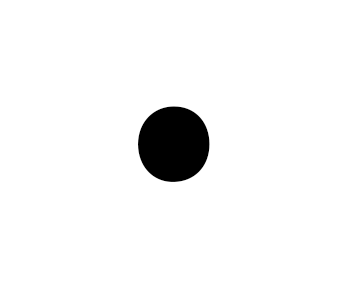
\includegraphics[width=0.5\textwidth]{graphs/fig1.png}
    \caption{\textit{tinyFaaS} Architecture}
    \label{img:systemdesign}
\end{figure}

In this section we will present the architecture of \textit{tinyFaaS}, which is shown in \cref{img:systemdesign}.
Its main components are a reverse proxy that acts as a CoAP proxy and load balancer, function handlers that execute the application code, and a management service to supervise the other components.
